\documentclass[11pt]{article}
\usepackage{latexsym}
\usepackage{amsmath}
\usepackage{amssymb}
\usepackage{amsthm}
\usepackage{epsfig}
\usepackage[tight]{subfigure}

\usepackage{amsmath}

\DeclareMathOperator*{\minimize}{min}
\DeclareMathOperator*{\maximize}{max}
\DeclareMathOperator*{\argmin}{arg\,min}
\DeclareMathOperator*{\argmax}{arg\,max}

\usepackage{algorithm}
 %on linux you may need to run sudo apt-get install texlive-full to install algorithm.sys
\usepackage{algorithmic}

\usepackage{verbatim}

%%%%%%%%%%%%%%%%%%%%%%%%%%%%%%%%%%%%%%%%%%
% Custom commands                        %
%%%%%%%%%%%%%%%%%%%%%%%%%%%%%%%%%%%%%%%%%%

\newcommand{\vc}[1]{\boldsymbol{#1}}
\newcommand{\adj}[1]{\frac{d J}{d #1}}
\newcommand{\chain}[2]{\adj{#2} = \adj{#1}\frac{d #1}{d #2}}

% mathcal
\newcommand{\Ac}{\mathcal{A}}
\newcommand{\Bc}{\mathcal{B}}
\newcommand{\Cc}{\mathcal{C}}
\newcommand{\Dc}{\mathcal{D}}
\newcommand{\Ec}{\mathcal{E}}
\newcommand{\Fc}{\mathcal{F}}
\newcommand{\Gc}{\mathcal{G}}
\newcommand{\Hc}{\mathcal{H}}
\newcommand{\Ic}{\mathcal{I}}
\newcommand{\Jc}{\mathcal{J}}
\newcommand{\Kc}{\mathcal{K}}
\newcommand{\Lc}{\mathcal{L}}
\newcommand{\Mc}{\mathcal{M}}
\newcommand{\Nc}{\mathcal{N}}
\newcommand{\Oc}{\mathcal{O}}
\newcommand{\Pc}{\mathcal{P}}
\newcommand{\Qc}{\mathcal{Q}}
\newcommand{\Rc}{\mathcal{R}}
\newcommand{\Sc}{\mathcal{S}}
\newcommand{\Tc}{\mathcal{T}}
\newcommand{\Uc}{\mathcal{U}}
\newcommand{\Vc}{\mathcal{V}}
\newcommand{\Wc}{\mathcal{W}}
\newcommand{\Xc}{\mathcal{X}}
\newcommand{\Yc}{\mathcal{Y}}
\newcommand{\Zc}{\mathcal{Z}}

% mathbb
\newcommand{\Ab}{\mathbb{A}}
\newcommand{\Bb}{\mathbb{B}}
\newcommand{\Cb}{\mathbb{C}}
\newcommand{\Db}{\mathbb{D}}
\newcommand{\Eb}{\mathbb{E}}
\newcommand{\Fb}{\mathbb{F}}
\newcommand{\Gb}{\mathbb{G}}
\newcommand{\Hb}{\mathbb{H}}
\newcommand{\Ib}{\mathbb{I}}
\newcommand{\Jb}{\mathbb{J}}
\newcommand{\Kb}{\mathbb{K}}
\newcommand{\Lb}{\mathbb{L}}
\newcommand{\Mb}{\mathbb{M}}
\newcommand{\Nb}{\mathbb{N}}
\newcommand{\Ob}{\mathbb{O}}
\newcommand{\Pb}{\mathbb{P}}
\newcommand{\Qb}{\mathbb{Q}}
\newcommand{\Rb}{\mathbb{R}}
\newcommand{\Sb}{\mathbb{S}}
\newcommand{\Tb}{\mathbb{T}}
\newcommand{\Ub}{\mathbb{U}}
\newcommand{\Vb}{\mathbb{V}}
\newcommand{\Wb}{\mathbb{W}}
\newcommand{\Xb}{\mathbb{X}}
\newcommand{\Yb}{\mathbb{Y}}
\newcommand{\Zb}{\mathbb{Z}}

% mathbf lowercase
\newcommand{\av}{\mathbf{a}}
\newcommand{\bv}{\mathbf{b}}
\newcommand{\cv}{\mathbf{c}}
\newcommand{\dv}{\mathbf{d}}
\newcommand{\ev}{\mathbf{e}}
\newcommand{\fv}{\mathbf{f}}
\newcommand{\gv}{\mathbf{g}}
\newcommand{\hv}{\mathbf{h}}
\newcommand{\iv}{\mathbf{i}}
\newcommand{\jv}{\mathbf{j}}
\newcommand{\kv}{\mathbf{k}}
\newcommand{\lv}{\mathbf{l}}
\newcommand{\mv}{\mathbf{m}}
\newcommand{\nv}{\mathbf{n}}
\newcommand{\ov}{\mathbf{o}}
\newcommand{\pv}{\mathbf{p}}
\newcommand{\qv}{\mathbf{q}}
\newcommand{\rv}{\mathbf{r}}
\newcommand{\sv}{\mathbf{s}}
\newcommand{\tv}{\mathbf{t}}
\newcommand{\uv}{\mathbf{u}}
\newcommand{\vv}{\mathbf{v}}
\newcommand{\wv}{\mathbf{w}}
\newcommand{\xv}{\mathbf{x}}
\newcommand{\yv}{\mathbf{y}}
\newcommand{\zv}{\mathbf{z}}

% mathbf uppercase
\newcommand{\Av}{\mathbf{A}}
\newcommand{\Bv}{\mathbf{B}}
\newcommand{\Cv}{\mathbf{C}}
\newcommand{\Dv}{\mathbf{D}}
\newcommand{\Ev}{\mathbf{E}}
\newcommand{\Fv}{\mathbf{F}}
\newcommand{\Gv}{\mathbf{G}}
\newcommand{\Hv}{\mathbf{H}}
\newcommand{\Iv}{\mathbf{I}}
\newcommand{\Jv}{\mathbf{J}}
\newcommand{\Kv}{\mathbf{K}}
\newcommand{\Lv}{\mathbf{L}}
\newcommand{\Mv}{\mathbf{M}}
\newcommand{\Nv}{\mathbf{N}}
\newcommand{\Ov}{\mathbf{O}}
\newcommand{\Pv}{\mathbf{P}}
\newcommand{\Qv}{\mathbf{Q}}
\newcommand{\Rv}{\mathbf{R}}
\newcommand{\Sv}{\mathbf{S}}
\newcommand{\Tv}{\mathbf{T}}
\newcommand{\Uv}{\mathbf{U}}
\newcommand{\Vv}{\mathbf{V}}
\newcommand{\Wv}{\mathbf{W}}
\newcommand{\Xv}{\mathbf{X}}
\newcommand{\Yv}{\mathbf{Y}}
\newcommand{\Zv}{\mathbf{Z}}

% bold greek lowercase
\newcommand{\alphav     }{\boldsymbol \alpha     }
\newcommand{\betav      }{\boldsymbol \beta      }
\newcommand{\gammav     }{\boldsymbol \gamma     }
\newcommand{\deltav     }{\boldsymbol \delta     }
\newcommand{\epsilonv   }{\boldsymbol \epsilon   }
\newcommand{\varepsilonv}{\boldsymbol \varepsilon}
\newcommand{\zetav      }{\boldsymbol \zeta      }
\newcommand{\etav       }{\boldsymbol \eta       }
\newcommand{\thetav     }{\boldsymbol \theta     }
\newcommand{\varthetav  }{\boldsymbol \vartheta  }
\newcommand{\iotav      }{\boldsymbol \iota      }
\newcommand{\kappav     }{\boldsymbol \kappa     }
\newcommand{\varkappav  }{\boldsymbol \varkappa  }
\newcommand{\lambdav    }{\boldsymbol \lambda    }
\newcommand{\muv        }{\boldsymbol \mu        }
\newcommand{\nuv        }{\boldsymbol \nu        }
\newcommand{\xiv        }{\boldsymbol \xi        }
\newcommand{\omicronv   }{\boldsymbol \omicron   }
\newcommand{\piv        }{\boldsymbol \pi        }
\newcommand{\varpiv     }{\boldsymbol \varpi     }
\newcommand{\rhov       }{\boldsymbol \rho       }
\newcommand{\varrhov    }{\boldsymbol \varrho    }
\newcommand{\sigmav     }{\boldsymbol \sigma     }
\newcommand{\varsigmav  }{\boldsymbol \varsigma  }
\newcommand{\tauv       }{\boldsymbol \tau       }
\newcommand{\upsilonv   }{\boldsymbol \upsilon   }
\newcommand{\phiv       }{\boldsymbol \phi       }
\newcommand{\varphiv    }{\boldsymbol \varphi    }
\newcommand{\chiv       }{\boldsymbol \chi       }
\newcommand{\psiv       }{\boldsymbol \psi       }
\newcommand{\omegav     }{\boldsymbol \omega     }

% bold greek uppercase
\newcommand{\Gammav     }{\boldsymbol \Gamma     }
\newcommand{\Deltav     }{\boldsymbol \Delta     }
\newcommand{\Thetav     }{\boldsymbol \Theta     }
\newcommand{\Lambdav    }{\boldsymbol \Lambda    }
\newcommand{\Xiv        }{\boldsymbol \Xi        }
\newcommand{\Piv        }{\boldsymbol \Pi        }
\newcommand{\Sigmav     }{\boldsymbol \Sigma     }
\newcommand{\Upsilonv   }{\boldsymbol \Upsilon   }
\newcommand{\Phiv       }{\boldsymbol \Phi       }
\newcommand{\Psiv       }{\boldsymbol \Psi       }
\newcommand{\Omegav     }{\boldsymbol \Omega     }


\newcommand{\handout}[5]{
  \noindent
  \begin{center}
  \framebox{
    \vbox{
      \hbox to 5.78in { {#1} \hfill #2 }
      \vspace{4mm}
      \hbox to 5.78in { {\Large \hfill #5  \hfill} }
      \vspace{2mm}
      \hbox to 5.78in { {\em #3 \hfill #4} }
    }
  }
  \end{center}
  \vspace*{4mm}
}

\newcommand{\lecture}[5]{\handout{#1}{#2}{#3}{#4}{#5}}
\newcommand{\collision}[0]{\mathrm{collision}}
\newcommand{\nocollision}[0]{\overline{\collision}}

\newcommand*{\QED}{\hfill\ensuremath{\square}}

\newtheorem{theorem}{Theorem}
\newtheorem{corollary}[theorem]{Corollary}
\newtheorem{lemma}[theorem]{Lemma}
\newtheorem{observation}[theorem]{Observation}
\newtheorem{proposition}[theorem]{Proposition}
\newtheorem{definition}[theorem]{Definition}
\newtheorem{claim}[theorem]{Claim}
\newtheorem{fact}[theorem]{Fact}
\newtheorem{assumption}[theorem]{Assumption}
\newtheorem{note}[theorem]{Note}

% 1-inch margins, from fullpage.sty by H.Partl, Version 2, Dec. 15, 1988.
\topmargin 0pt
\advance \topmargin by -\headheight
\advance \topmargin by -\headsep
\textheight 8.9in
\oddsidemargin 0pt
\evensidemargin \oddsidemargin
\marginparwidth 0.5in
\textwidth 6.5in

\parindent 0in
\parskip 1.5ex
%\renewcommand{\baselinestretch}{1.25}

\begin{document}

\lecture{Statistical Techniques in Robotics (16-831, S21)}{Lecture \#12
  (Monday, March 15)}{Lecturer: Kris Kitani}{Scribes: Abhinav Agarwalla, Kshitij Goel}{Bandits (Explore-Exploit), UCB}

\section{Review}
In the previous lecture, we finished learning about AdaBoost algorithm and started
understanding the Multi-Armed Bandit problem and one algorithm (Explore-Exploit) for it.

\subsection{Adaboost}
\subsubsection{PAC Learning Model}
The PAC learning model is a theoretical framework to answer two questions:
\begin{enumerate}
    \item What is the optimal dataset size to obtain good generalization?
    \item What is the computational cost of learning?
\end{enumerate}

\subsubsection{Boosting}
The theorem based on \cite{schapire1990strength} suggests that a weak PAC learner can be called
multiple times to generate a sequence of hypothesis with a different subset of $\Dv$ which
can be combined to form a single strong PAC learner. This process is called \textit{boosting}.

Adaboost~\cite{freund1997decision} is a specific learning algorithm in the class of boosting algorithms. In previous online learning methods, one receives new data points at every time instant. In Adaboost, we receive \textit{weak learners} instead of data points. The final prediction rule is a weighted sum of learner predictions upto the current time $T$. Since we have $T$ weak learner at time step $T$, we just use the 'number of weak learners' terminology over time steps. The Adaboost algorithm is detailed in Algorithm \ref{algo:adaboost}.

\begin{algorithm}
\caption{Adaboost}
\label{algo:adaboost}
\begin{algorithmic}[1]
\STATE Input: Dataset $\Dv =\{\xv_n, y_n\}_{n=1}^{N}$, where feature vector $\xv_n \in \mathbb{R}^M$ and label $y \in \{0, 1\}$
\STATE Input: Weight vector $\{w^{(0)}\}_{n=1}^{N}$ initialised uniformly
\STATE Input: Number of weak learners $T$ 
\FOR{$t=1,\;\cdots,\;T$}
\STATE $\pv^{(t)} = \wv^{(t-1)}/(\sum_n w_n^{(t-1)})$ 
\STATE $h^{(t)} = \mathtt{WEAKLEARNER}(\Dv, \pv^{(t)})$  \hfill $\triangleright$ Prediction Step
\STATE $\epsilon^{(t)} = \sum_n p^t_n |h^{(t)}(\xv_n) - y_n|$
\STATE $\beta^{(t)} = \frac{\epsilon^{(t)}}{1-\epsilon^{(t)}}$
\STATE $w_n^{(t)} = w_n^{(t-1)}\beta^{1-|h^{(t)}(\xv_n^{(t)}-y_n^{(t)}|} \qquad \forall n$ \hfill $\triangleright$ Weight Update Step
\ENDFOR
\STATE $h_F(\xv) = \mathbbm{1}\left[\sum_{t=1}^T (log(\frac{1}{\beta^{(t)}}))h^{(t)}(\xv) \ge \frac{1}{2} \sum_{t=1}^{T} log(\frac{1}{\beta^{(t)}})\right]$
\end{algorithmic}
\end{algorithm}

\subsection{Multi-Armed Bandits}
\begin{enumerate}
    \item \textbf{One-Shot Feedback}: This is because one action from the player leads to one
    reward and selecting any particular action does not change the state at the next time-step.
    \item \textbf{Exhaustive Feedback}: The player can pull all the arms for the duration of the
    game. The state and action spaces are finite.
    \item \textbf{Evaluative Feedback}: The player receives a reward sampled from the underlying
    unknown reward distributions at each time-step.
\end{enumerate}
Based on this type of feedback, the goal is to maximize the total reward the player receives over
a horizon. Applications of the MAB problem include: A/B testing (figuring out which advertisement to display based on how
the user interacts with the advertisement experience), robotic grasping (which way should the robot pick up
an object), medical treatment (treating patient's health status as reward, advise treatment).
\subsubsection{Explore-exploit algorithm}
Assuming a stochastic bandit, how should the player pull the arms if they have only $T$ rounds? The
Explore-Exploit algorithm aims at answering this question. At a high-level, the algorithm proceeds in two
phases:
\begin{enumerate}
    \item \textbf{Explore Phase}: Pull each arm $M$ times to estimate the mean reward.
    \item \textbf{Exploit Phase}: Keep pulling the arm with the highest expected mean reward until $T$.
\end{enumerate}
%This section serves as a review of the previous lecture and any other context required to frame the content of the current lecture. 

%You may format the scribes in any way you like, aside from changing font style, size and page format. Please use subsections and paragraphs to increase the readability of your notes.

%Length requirement 1-2 pages.

\section{Summary}

\subsection{Multi-Armed Bandit: Explore-Exploit}
The algorithm for the Explore-Exploit algorithm is shown in Alg. \ref{algo:explore-exploit}.
\begin{algorithm}
\caption{Explore-Exploit}
\label{algo:explore-exploit}
\begin{algorithmic}[1]
\FOR{$k=1 \rightarrow K$}
\FOR{$m=1 \rightarrow M$}
\STATE $a = k$
\STATE $\mathtt{Receive}(r)$
\STATE $\hat{\mu}_k = \hat{\mu}_k + \frac{r}{M}$
\ENDFOR
\ENDFOR
\FOR{$t = KM \rightarrow T$}
\STATE $a^{(t)} = \arg \max_{k'} \hat{\mu}_{k'}$
\STATE $\mathtt{Receive}(r^{(t)})$
\ENDFOR
\end{algorithmic}
\end{algorithm}

\theorem{\normalfont \textbf{Hoeffding's Inequality} Consider a one-dimension distribution $\nu$ with expectation
$\mu$, where any sample $r \sim \nu$ is bounded such that $r \in [0, 1]$. Given $T$ i.i.d samples, $\{ r^{(t)} \}_{t=1}^T$, we have that for any $\epsilon$: $$p \left( \left| \sum_{t=1}^T \frac{r^{(t)}}{T} - \mu \right| \geq \epsilon \right) \leq 2 e^{-2T\epsilon^2}$$ }

\normalfont
Intuitively, this inequality means that the estimate of the mean gets better with the more samples are available. We will use this inequality in the
regret bound derivation for the Explore-Exploit algorithm.

\subsubsection{Regret Analysis}
%Note that the Hoeffding's Inequality can also be written as
%\[
%p \left( \left| \sum_{t=1}^T \frac{r^{(t)}}{T} - \mu \right| < \epsilon \right) %\geq 1 - 2 e^{-2T\epsilon^2}
%\]

\begin{figure}
    \centering
    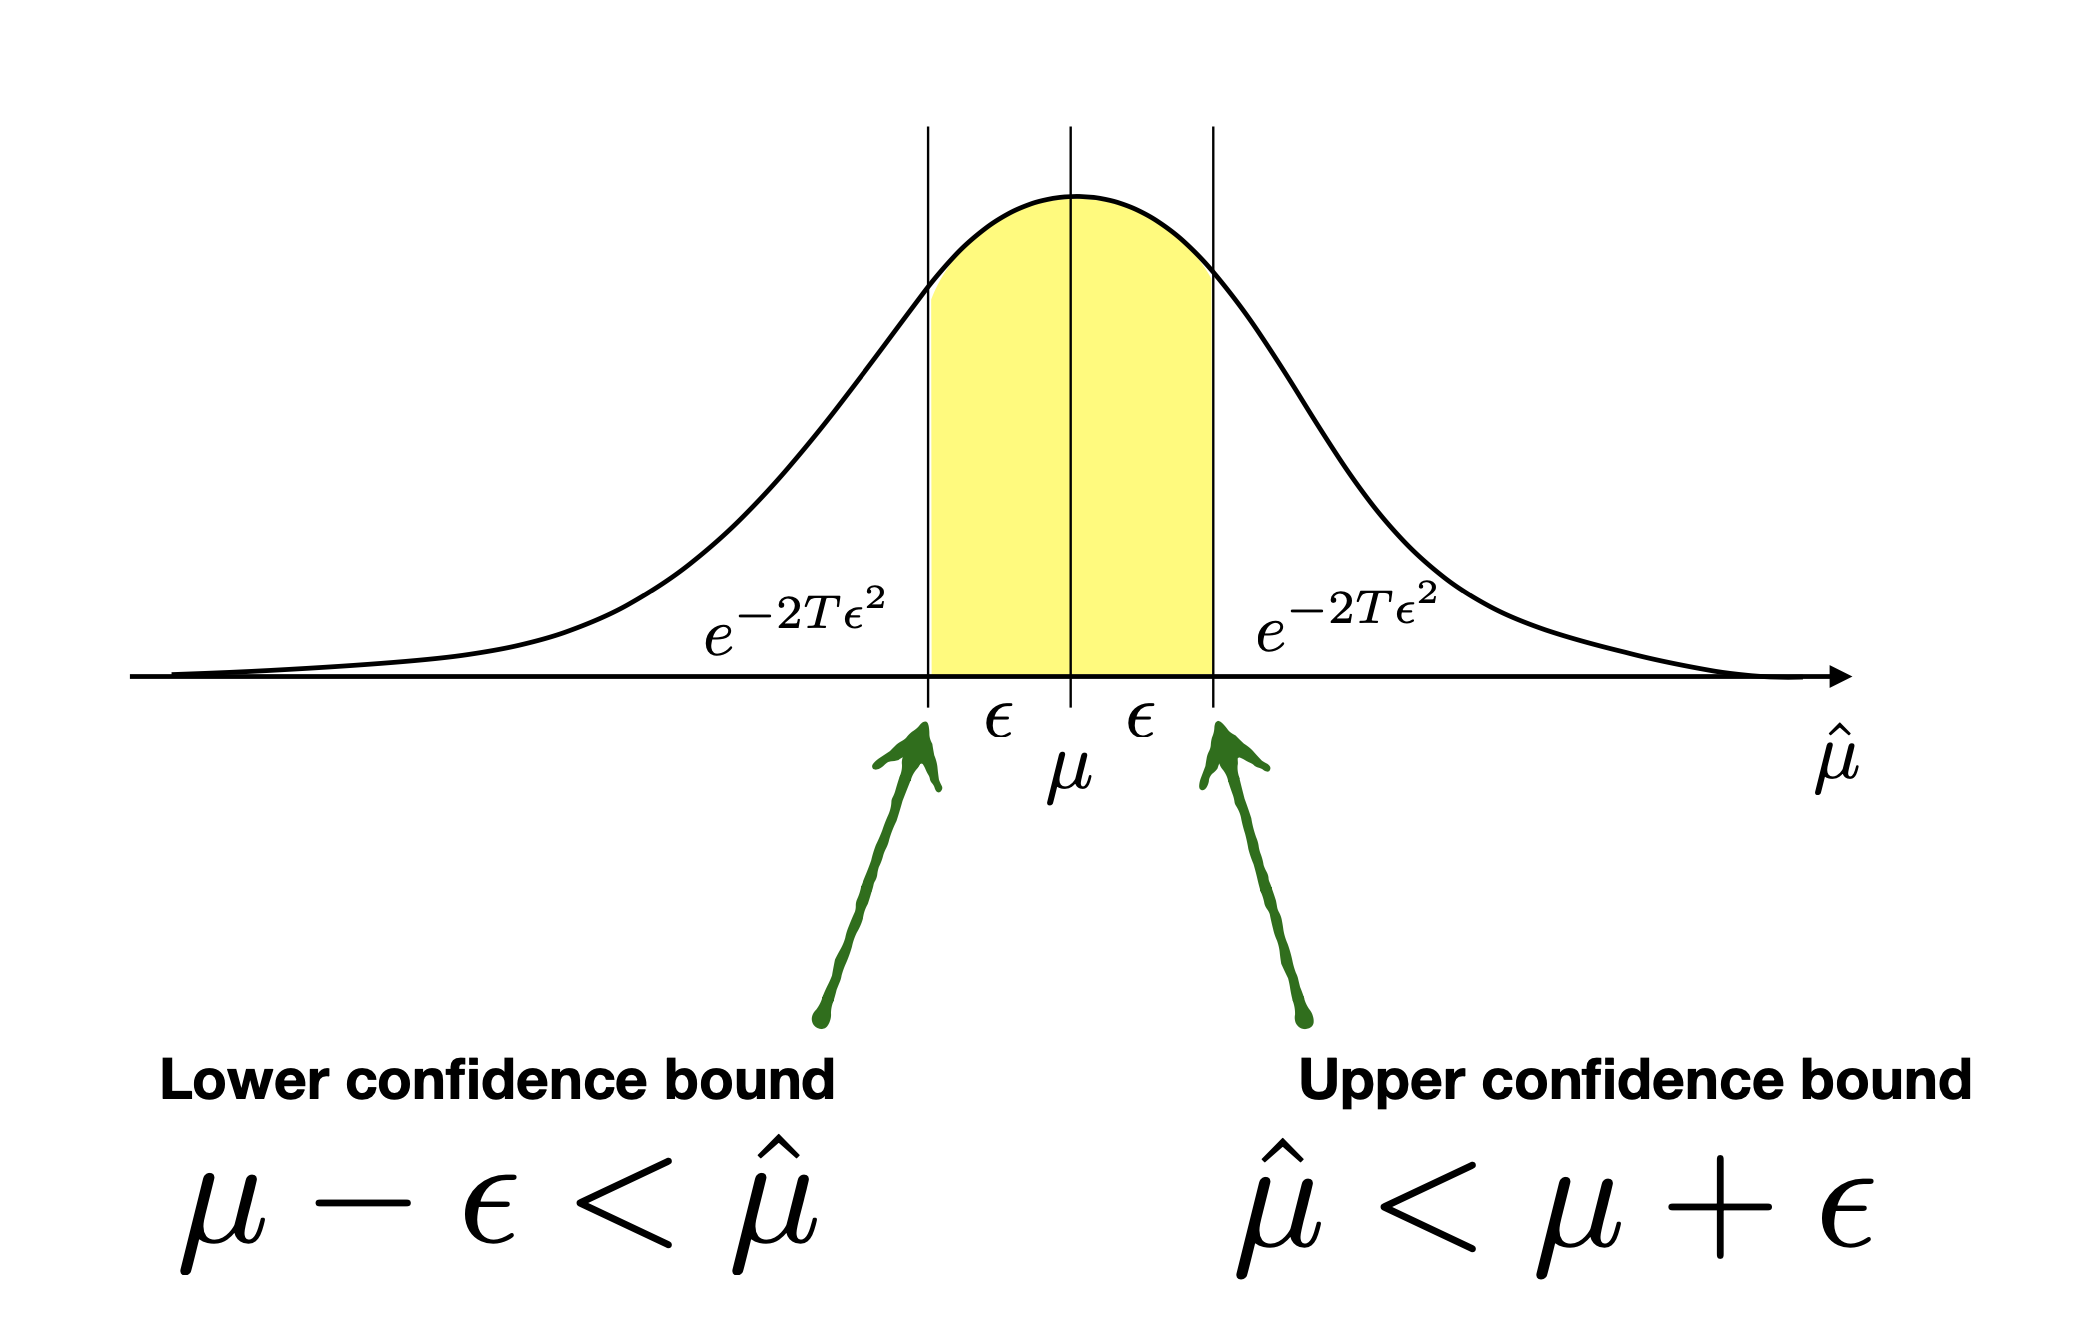
\includegraphics[width=0.5\textwidth]{images/ucb_lcb.png}
    \caption{Illustrations of the definitions for the Lower Confidence Bound (LCB) and Upper Confidence Bound (UCB).}
    \label{fig:ucb_lcb}
\end{figure}

We will derive the regret bound in two steps: first for the exploration phase
and then for the exploitation phase.

\paragraph{Exploration Phase}
For the exploration phase, the bound is $\mathcal{O}(KM)$ because it requires $KM$
pulls and still gets no reward. $$ R_{\text{explore}} \leq \mathcal{O}(KM)$$

\paragraph{Exploitation Phase}
For the exploitation phase, we define the potential function using the fact
that if we pulled the wrong arm (i.e. not the true best arm), that means
our estimate of the best arm was wrong. Formally, our potential is defined
as
\[
\hat{\mu}_{\hat{k}} \geq \hat{\mu}_{k^*}
\]

Now, we derive the upper and lower bounds of this potential.

\textbf{Upper Bound} For the upper bound, we can use the Upper Confidence Bound (UCB) (illustrated
in Fig. \ref{fig:ucb_lcb}):
\begin{align*}
\hat{\mu}_{\hat{k}} &\leq \mu_{\hat{k}} + \epsilon\\
&\leq \mu_{\hat{k}} + \sqrt{\frac{\log{2/\delta}}{2M}}
\end{align*}

\textbf{Lower Bound} For the lower bound, we can use the Lower Confidence Bound (UCB) (illustrated
in Fig. \ref{fig:ucb_lcb}):
\begin{align*}
\hat{\mu}_{\hat{k}} &\geq \mu_{k^*} - \epsilon\\
&\geq \mu_{k^*} - \sqrt{\frac{\log{2/\delta}}{2M}}
\end{align*}

\textbf{Combining Lower and Upper Bounds} We can combine these bounds as after some algebra derive the regret bound for the exploitation
phase.
\begin{align*}
\mu_{\hat{k}} + \sqrt{\frac{\log (2/\delta)}{2M}} &\geq \mu_{k^*} - \sqrt{\frac{\log (2/\delta)}{2M}}\\
\mu_{k^*} - \mu_{\hat{k}} &\leq 2 \sqrt{\frac{\log (2/\delta)}{2M}}\\
R_{\text{exploit}} &= \sum_{t=KM+1}^T (\mu_{k^*}^{(t)} - \mu_{\hat{k}}^{(t)}) \leq (T - KM) \cdot 2 \sqrt{\frac{\log (2/\delta)}{2M}}
\end{align*}

\paragraph{Combining Exploration and Exploitation Bounds}
We now have expressions for the regret bounds for the explore and exploit phases. The sum gives
us the final expression for the regret of the explore-exploit algorithm.

\begin{align*}
    R_{\text{explore-exploit}} &= R_{\text{explore}} + R_{\text{exploit}}\\
    &= KM + (2T - KM) \cdot \sqrt{\frac{1}{M}}\\
    \leq KM + 2T \cdot \sqrt{\frac{1}{M}}
\end{align*}

Observe that the regret is linear in $T$, which is what we do not want. If we want our
algorithm to be no-regret, we want the regret to grow sub-linearly. So, we can choose
$M$ in a way to make the regret sub-linear. We take the derivative of RHS and set it to zero.
\begin{align*}
    0 &= \frac{d}{dM} \Big\{ KM + 2T \cdot \sqrt{\frac{1}{M}} \Big\}\\
    0 &= K - TM^{-3/2}\\
    M &= \left( \frac{T}{K} \right)^{2/3}\\
\end{align*}

Plugging this optimal $M$ into our regret bound expression, we get:
\begin{align*}
    R &= R_{\text{explore}} + R_{\text{exploit}}\\
    &\leq KM + 2T \cdot \sqrt{\frac{1}{M}}\\ 
    &= K \left( \frac{T}{K} \right)^{2/3} + 2T \sqrt{\left( \frac{T}{K}\right)^{-2/3}}\\
    &= K \left( \frac{T}{K} \right)^{2/3} + 2T \left( \frac{T}{K}\right)^{-1/3}\\
    &= K^{1/3}T^{2/3} + 2T^{2/3}K^{1/3}\\
    &= 3K^{1/3}T^{2/3}\\
    &= \mathcal{O}(K^{1/3}T^{2/3})
\end{align*}

Thus, the regret bound for the Explore-Exploit algorithm is $R = \mathcal{O}(K^{1/3}T^{2/3})$. Note that this
is a sub-linear regret bound and that the total number of pulls $T$ is assumed to be known.

\subsection{Multi-Armed Bandit: Upper Confidence Bound}

Upper Confidence Bound (UCB) is another algorithm to solve a context-free bandit problem. UCB is an optimistic learner where the arm $k(t)$ with the largest mean reward ($\hat{\mu}_{k}$) plus a confidence term is picked. The algorithm is detailed in Algo.~\ref{algo:ucb}.

\begin{algorithm}[H]
\caption{Upper Confidence Bound (UCB)}
\label{algo:ucb}
\begin{algorithmic}[1]
% \STATE Input: Time horizon $T$
\FOR{$t=1 \rightarrow T$}
\IF{$t \le K$}
\STATE $k = t$ \hfill $\triangleright$ Initially pull each arm once (exploration)
\ELSE
\STATE $k = \argmax_{k'} \left(\hat{\mu}_{k'
} + \sqrt{\frac{\log(2T/\delta')}{2T_{k'}^{(t)}}} \right)$ \hfill $\triangleright$ upper confidence
\ENDIF
\STATE $\mathtt{RECEIVE}(r^{(t)})$
\STATE $T_k^{(t)} = T_k^{(t')} + 1$  \hfill $\triangleright$ update pull counter
\STATE $\hat{\mu}_{k} = \frac{1}{T_k^{(t)}}\left(\hat{\mu}_{k}(T_k^{(t)} - 1) + r^{(t)}\right)$ \hfill $\triangleright$ update mean reward for k
\ENDFOR
\end{algorithmic}
\end{algorithm}

\subsubsection{Understanding confidence term}
The confidence term is obtained using Hoeffding's inequality and depends on the number of pulls of a particular arm $T_{k'}^{(t)}$, total pulls $T$ and $\delta$. So, as the game progresses and the number of pulls increase, the learner becomes more confident and the confidence term reduces.

\theorem{\normalfont\textbf{Union Bound} The probability that at least one of the events happens is no
greater than the sum of the probabilities of the individual events. Mathematically, $p(\bigcup_i x_i) \le \sum_i p(x_i)$, where $x_i$'s are events.}\\
\normalfont\textbf{Proof Sketch} For two events $x_1$ and $x_2$, $p(x_1 \cup x_2) = p(x_1) + p(x_2) - p(x_1 \cap x_2)$\\
$p(x_1 \cup x_2) \le p(x_1) + p(x_2)$\\
The same logic can be extended to arbitary $n$ events.

Now using Hoeffding inequality (Theorem 1) and Union bound (Theorem 2), 
$$p(\bigcup_{t=1}^T\left[|\hat{\mu}_k^{(t)} - \mu_k| > \sqrt{\frac{\log(2/\delta)}{2T_{k}^{(t)}}} \right]) \le \sum_{t=1}^Tp\left(|\hat{\mu}_k^{(t)} - \mu_k| > \sqrt{\frac{\log(2/\delta)}{2T_{k}^{(t)}}}\right) \le T\delta = \delta'$$

Thus for the union event, the confidence interval becomes:
$$\epsilon' = \sqrt{\frac{\log(2T/\delta')}{2T_{k}^{(t)}}}$$

\subsubsection{Regret Bound}

For UCB, the regret bound comes out to $\mathcal{O}(\sqrt{KT})$. Next, we will derive the regret bound.

% % \theorem{\normalfont\textbf{Re}

\textbf{Base Inequality} We first define the base inequality which is akin to potential function in some sense. If the learner selects a non-optimal arm $k \neq k^*$ where $k^*$ is the optimal arm, we can say that the estimated mean plus the confidence term for that arm is higher than the same for the optimal arm (from prediction step, line 5 in Algo.~\ref{algo:ucb}). Mathematically, :
$$\hat{\mu}_k^{(t)} + \sqrt{\frac{\log(2T/\delta')}{2T_{k}^{(t)}}} \ge \hat{\mu}_{k^*}^{(t)} + \sqrt{\frac{\log(2T/\delta')}{2T_{k^*}^{(t)}}}$$

\textbf{Upper Bound} We wish to obtain a upper bound on the LHS of previous inequality. From Heoffding's inequality, $|\hat{\mu}^{(t)} - \mu| \le \epsilon'$ or $\hat{\mu}^{(t)} \le \epsilon' + \mu$ since we interested in upper bound. Using this, we have: 
$$\hat{\mu}_k^{(t)} \le \mu_k + \sqrt{\frac{\log(2T/\delta')}{2T_{k}^{(t)}}}$$
$$\mu_k + 2\sqrt{\frac{\log(2T/\delta')}{2T_{k}^{(t)}}} \ge \hat{\mu}_k^{(t)} + \sqrt{\frac{\log(2T/\delta')}{2T_{k}^{(t)}}}$$

\textbf{Lower Bound} We wish to obtain a upper bound on the RHS of the base inequality. From Heoffding's inequality, $|\hat{\mu}^{(t)} - \mu| \le \epsilon'$ or $\hat{\mu}^{(t)} \ge \mu - \epsilon'$ since we interested in lower bound.
$$\hat{\mu}_{k^*}^{(t)} \ge \mu_{k^*} - \sqrt{\frac{\log(2T/\delta')}{2T_{k^*}^{(t)}}}$$
$$\hat{\mu}_{k^*}^{(t)} + \sqrt{\frac{\log(2T/\delta')}{2T_{k^*}^{(t)}}} \ge \mu_{k^*} - \sqrt{\frac{\log(2T/\delta')}{2T_{k^*}^{(t)}}} + \sqrt{\frac{\log(2T/\delta')}{2T_{k^*}^{(t)}}}$$
$$\hat{\mu}_{k^*}^{(t)} + \sqrt{\frac{\log(2T/\delta')}{2T_{k^*}^{(t)}}} \ge \mu_{k^*}$$
\textbf{Combining Bounds} 
$$\mu_k + 2\sqrt{\frac{\log(2T/\delta')}{2T_{k}^{(t)}}} \ge \mu_{k^*}$$
$$\mu_{k^*} - \mu_k \le 2\sqrt{\frac{\log(2T/\delta')}{2T_{k}^{(t)}}}$$
The above equation is for just one pull $k$. We are pulling an arm $k(t)$ at each time instant $t$. Thus,
$$\mathcal{R}_{UCB} = \sum_{t=1}^T (\mu_{k^*} - \mu_{k^{(t)}})$$
$$ = \sum_{t=1}^T 2\sqrt{\frac{\log(2T/\delta')}{2T_{k^{(t)}}^{(t)}}}$$
$$ = \sqrt{2\log(2T/\delta')} \sum_{t=1}^T \sqrt{\frac{1}{T_{k^{(t)}}^{(t)}}}$$
$$ = \sqrt{2\log(2T/\delta')} \sum_{t=1}^T \sum_{j=1}^K \mathbbm{1}[k^{(t)} = j]\sqrt{\frac{1}{T_{j}^{(t)}}}$$
$$ = \sqrt{2\log(2T/\delta')} \sum_{j=1}^K \sum_{t=1}^T \mathbbm{1}[k^{(t)} = j]\sqrt{\frac{1}{T_{j}^{(t)}}}$$
$$ = \sqrt{2\log(2T/\delta')} \sum_{j=1}^K \sum_{t=1}^{T_j^{(T)}} \sqrt{\frac{1}{t}}$$

There are two mathematical inequalities required to derive the bound.
\fact{\normalfont Summation Bound: $\sum_{t=1}^{T}\sqrt{\frac{1}{t}} \le 2\sqrt{T}$}\\
Proof. $\sum_{t=1}^{T}\sqrt{\frac{1}{t}} = 1 + \sum_{t=2}^{T}\sqrt{\frac{1}{t}} \le 1 + \int_{t=1}^{T}\sqrt{\frac{1}{t}}dt$ \hfill 
(as $\sum_{t=n+1}^T \frac{1}{\sqrt{T}} \le \int_{t=n}^T \frac{1}{\sqrt{T}}dt)$\\
$ = 1 + 2\sqrt{T} - 2 = 2\sqrt{T} - 1 \le 2\sqrt{T}$

\theorem{\normalfont\textbf{Jensen's Inequality} If and only if $f$ is a convex function, $f(\sum_np_nx_n) \le \sum_np_nf(x_n)$. Equivalently, if $f$ is concave, $\sum_np_nf(x_n) \le f(\sum_np_nx_n)$.}

\normalfont
Continuing with the derivation, 
$$\mathcal{R}_{UCB} \le \sqrt{2\log(2T/\delta')} \sum_{j=1}^K \sum_{t=1}^{T_j^{(T)}} \sqrt{\frac{1}{t}}$$
$$\le \sqrt{2\log(2T/\delta')} \sum_{j=1}^K 2\sqrt{T_j^{(T)}} \qquad \text{(Using Fact 3)}$$
$$\le \sqrt{8\log(2T/\delta')} K \left(\frac{1}{K}\sum_{j=1}^K \sqrt{T_j^{(T)}} \right)$$
$$\le \sqrt{8\log(2T/\delta')} K \left( \sqrt{\frac{1}{K}\sum_{j=1}^K T_j^{(T)}} \right)  \qquad \text{(Using Jensen's inequality)}$$
$$= \sqrt{8\log(2T/\delta')} K \left( \sqrt{\frac{T}{K}} \right)$$
$$= \sqrt{8\log(2T/\delta')} \sqrt{TK} \approx \mathcal{O}(\sqrt{TK})$$

In the slides, the constant term misses the factor of $\sqrt{8}$.

The regret bound for UCB is better than Explore-Exploit. This is because it starts exploiting earlier and continues exploring.

%\section*{References}
%Include your references here. Please cite any resources you found useful.	
%Populate the refs.bib file or list your references manually. Be consistent in formatting!
\newpage
{
\bibliography{refs}
\bibliographystyle{abbrv}
}

%\section{Appendix}
%This section provides any relevant background material that was not covered in the lectures, but was found to be useful for understanding the material. 
%For example, derivations, theory underlying techniques employed, etc. 

%Additionally, this section can summarizes applications or extensions of these techniques found in the literature. 

\end{document} % Done!


